\chapter{\ifproject%
\ifenglish Project Structure and Methodology\else โครงสร้างและขั้นตอนการทำงาน\fi
\else%
\ifenglish Project Structure\else โครงสร้างของโครงงาน\fi
\fi
}

ในบทนี้จะกล่าวถึงหลักการ และการออกแบบระบบ

\makeatletter

% \renewcommand\section{\@startsection {section}{1}{\z@}%
%                                    {13.5ex \@plus -1ex \@minus -.2ex}%
%                                    {2.3ex \@plus.2ex}%
%                                    {\normalfont\large\bfseries}}

\makeatother
%\vspace{2ex}
% \titleformat{\section}{\normalfont\bfseries}{\thesection}{1em}{}
% \titlespacing*{\section}{0pt}{10ex}{0pt}

\section{ภาพรวมระบบ (System Overview)}
ระบบที่พัฒนาขึ้นมีวัตถุประสงค์เพื่อวัดความสูงของต้นไม้ โดยอาศัยการผสานเทคโนโลยี Ultra-Wideband (UWB) ร่วมกับอากาศยานไร้คนขับ (UAV) และการประมวลผลภาพถ่ายทางอากาศเพื่อสร้างแบบจำลองสามมิติ (3D Reconstruction) ซึ่งใช้เป็นค่ามาตรฐานอ้างอิงในการประเมินความแม่นยำของระบบ

\subsection{ภาพรวมการทำงานของระบบ}
ระบบแบ่งการทำงานออกเป็น 2 กระบวนการหลัก ได้แก่ (1) การวัดระยะด้วย UWB ร่วมกับเซ็นเซอร์ VPS และ (2) การสร้างแบบจำลองสามมิติจากภาพถ่ายทางอากาศ

ในกระบวนการที่หนึ่ง อุปกรณ์ Tag ที่ติดตั้งบนโดรนจะสื่อสารกับ Anchor บนพื้นดินเพื่อวัดระยะทางด้วยเทคนิค Time of Flight (ToF) ขณะที่โดรนลอยตัวเหนือยอดไม้ โดยใช้เซ็นเซอร์ VPS วัดระยะจากโดรนถึงยอดไม้ จากนั้นนำค่าที่ได้มาคำนวณความสูงของต้นไม้

ในกระบวนการที่สอง โดรนจะเก็บภาพถ่ายทางอากาศของพื้นที่เป้าหมายในช่วงเวลาที่ใกล้เคียงกัน แล้วนำไปประมวลผลด้วย WebODM เพื่อสร้าง 3D Point Cloud และแบบจำลอง DSM/DTM ซึ่งใช้คำนวณความสูงของต้นไม้ (CHM) เพื่อเป็นค่ามาตรฐานอ้างอิง

\subsection{องค์ประกอบของระบบ}
ระบบประกอบด้วยองค์ประกอบหลัก 4 ส่วน ได้แก่
\begin{itemize}
    \item \textbf{ระบบ UWB:} ใช้วัดระยะระหว่าง Tag บนโดรน และ Anchor บนพื้นดิน
    \item \textbf{อากาศยานไร้คนขับ (UAV):} ใช้สำหรับติดตั้ง Tag ควบคุมตำแหน่ง และเก็บภาพถ่าย
    \item \textbf{สถานีภาคพื้น:} รวบรวมข้อมูลจากระบบ UWB ทำการจัดรูปแบบข้อมูล และบันทึกลงไฟล์ CSV เพื่อใช้ในการวิเคราะห์และเปรียบเทียบผล
    \item \textbf{ระบบประมวลผลภาพ:} ใช้ WebODM สำหรับสร้างแบบจำลองสามมิติ
\end{itemize}

\subsection{การไหลของข้อมูล (Data Flow)}
การทำงานของระบบมีลักษณะเป็นการประมวลผลแบบขนาน (Parallel Processing) โดยสามารถแบ่งออกเป็น 2 กระบวนการหลัก ได้แก่ การวัดระยะด้วยเทคโนโลยี UWB ร่วมกับเซ็นเซอร์ VPS และการสร้างแบบจำลองสามมิติจากภาพถ่ายทางอากาศ ซึ่งมีรายละเอียดดังนี้

\begin{enumerate}
    \item \textbf{กระบวนการวัดระยะด้วย UWB และ VPS}
    \begin{itemize}
        \item วัดระยะในแนวดิ่งจากตัวโดรนถึงยอดไม้โดยใช้เซ็นเซอร์ Vision Positioning System (VPS)
        \item วัดระยะห่างระหว่างอุปกรณ์ Tag และ Anchor โดยใช้เทคนิค Time of Flight (ToF) โดยรักษาระดับความสูงเดิมและปรับตำแหน่งในแนวราบเพื่อหลีกเลี่ยงการบังสัญญาณ
        \item นำค่าระยะทางที่ได้มาคำนวณเพื่อประมาณค่าความสูงของต้นไม้
        \item บันทึกข้อมูลระยะทางและผลการคำนวณในรูปแบบไฟล์ CSV เพื่อใช้ในการวิเคราะห์ภายหลัง
    \end{itemize}

    \item \textbf{กระบวนการสร้างแบบจำลองสามมิติ}
    \begin{itemize}
        \item เก็บภาพถ่ายทางอากาศของพื้นที่เป้าหมาย
        \item นำภาพถ่ายที่ได้ไปประมวลผลด้วยซอฟต์แวร์ WebODM
        \item สร้างแบบจำลองสามมิติในรูปแบบ 3D Point Cloud รวมถึงแบบจำลองความสูงเชิงเลข (DSM และ DTM)
        \item คำนวณค่าความสูงของต้นไม้จากข้อมูลแบบจำลอง (Canopy Height Model: CHM)
    \end{itemize}

    \item นำค่าความสูงของต้นไม้ที่ได้จากทั้งสองกระบวนการมาเปรียบเทียบกัน โดยใช้ค่าที่ได้จากแบบจำลองสามมิติ (3D Point Cloud) เป็นค่ามาตรฐานอ้างอิง เพื่อประเมินความแม่นยำของระบบ
\end{enumerate}

\begin{figure}[H]
  \centering
  \resizebox{0.95\textwidth}{!}{
  \begin{tikzpicture}[node distance=1.6cm and 3cm]

  % styles
  \tikzstyle{process} = [rectangle, minimum width=4.5cm, minimum height=1cm, text centered, align=center, draw=black]
  \tikzstyle{startstop} = [ellipse, minimum width=3.5cm, minimum height=1cm, text centered, draw=black]
  \tikzstyle{arrow} = [thick,->,>=stealth]

  % start
  \node (start) [startstop] {Start System};

  % split
  \node (split) [process, below of=start] {เริ่มการเก็บข้อมูล};

  % LEFT PIPELINE (UWB)
  \node (uwb1) [process, below left=of split] {วัดระยะจากโดรนถึงยอดไม้ (VPS)};
  \node (uwb2) [process, below of=uwb1] {วัดระยะด้วย UWB (Tag-Anchor)};
  \node (uwb3) [process, below of=uwb2] {คำนวณความสูงต้นไม้ \\ (ผลต่างระหว่างระยะ UWB และ VPS)};

  % RIGHT PIPELINE (Photogrammetry)
  \node (img1) [process, below right=of split] {เก็บภาพถ่ายทางอากาศ};
  \node (img2) [process, below of=img1] {ประมวลผลด้วย WebODM \\ (3D Point Cloud / DSM / DTM)};
  \node (img3) [process, below of=img2] {คำนวณความสูงต้นไม้ \\ จาก Point Cloud};

  % merge
  \node (compare) [process, below=7cm of split] {เปรียบเทียบค่าความสูง \\ (UWB vs 3D Model)};
  \node (end) [startstop, below of=compare] {End};

  % arrows
  \draw [arrow] (start) -- (split);

  \draw [arrow] (split) -| (uwb1);
  \draw [arrow] (uwb1) -- (uwb2);
  \draw [arrow] (uwb2) -- (uwb3);
  \draw [arrow] (uwb3) |- (compare);

  \draw [arrow] (split) -| (img1);
  \draw [arrow] (img1) -- (img2);
  \draw [arrow] (img2) -- (img3);
  \draw [arrow] (img3) |- (compare);

  \draw [arrow] (compare) -- (end);

  \end{tikzpicture}
  }
  \caption{แผนภาพกระบวนการทำงานแบบขนานสำหรับการประมาณความสูงของต้นไม้โดยใช้ UWB และโฟโตแกรมเมทรี}
  \label{fig:parallel-system}
\end{figure}

\subsection{ข้อจำกัดของระบบ (System Limitations)}
แม้ว่าระบบจะถูกออกแบบมาเพื่อให้มีความแม่นยำสูง แต่ยังมีข้อจำกัดบางประการ ได้แก่
\begin{itemize}
    \item ความคลาดเคลื่อนจากการจัดตำแหน่งโดรนให้ตรงกับ Anchor ในแนวดิ่ง
    \item ผลกระทบจากสภาพแวดล้อม เช่น ความหนาแน่นของต้นไม้ ซึ่งอาจทำให้เกิดสัญญาณสะท้อน (Multipath) หรือสภาวะ Non-Line-of-Sight (NLOS)
    \item ความไม่เสถียรของโดรนขณะลอยตัว ซึ่งอาจส่งผลต่อความคลาดเคลื่อนของค่าระยะทางที่วัดได้
    \item ความคลาดเคลื่อนของแบบจำลอง 3 มิติที่ใช้เป็นค่ามาตรฐานอ้างอิง
\end{itemize}

\section{โครงสร้างฮาร์ดแวร์ของระบบ}
\begin{enumerate}
    \item \textbf{ESP32 UWB:} ทำหน้าที่เป็นอุปกรณ์ Tag และ Anchor สำหรับการวัดระยะทาง โดยอาศัยหลักการ Time of Flight (ToF) ในการคำนวณระยะห่างระหว่างอุปกรณ์ ซึ่งค่าระยะทางที่ได้จะถูกนำไปใช้ในการคำนวณความสูงของต้นไม้
    \item \textbf{โดรน DJI M30T:} ใช้เป็นแพลตฟอร์มสำหรับติดตั้งโมดูล UWB และควบคุมตำแหน่งให้ลอยตัวเหนือยอดต้นไม้ นอกจากนี้ยังใช้เซ็นเซอร์ของโดรนในการวัดระยะจากตัวโดรนถึงยอดไม้ (VPS) และใช้กล้องสำหรับบันทึกภาพถ่ายทางอากาศ รวมถึงการปรับตำแหน่งในแนวราบเพื่อดำเนินการวัดระยะด้วย UWB
    \item \textbf{Laptop Computer:} ใช้เป็นสถานีภาคพื้นสำหรับรับข้อมูลจากอุปกรณ์ UWB ทำการจัดรูปแบบและบันทึกข้อมูล รวมถึงประมวลผลข้อมูลเพื่อคำนวณความสูงของต้นไม้
    \item \textbf{โครงยึดอุปกรณ์ (3D Printing):} ใช้สำหรับติดตั้งโมดูล UWB Tag บนโดรน โดยออกแบบให้มีน้ำหนักเบา มีความแข็งแรง และไม่รบกวนการทำงานของเซ็นเซอร์หรือกล้องของโดรน
\end{enumerate}

\begin{figure}[htbp]
    \centering
    \begin{minipage}{0.45\textwidth}
        \centering
        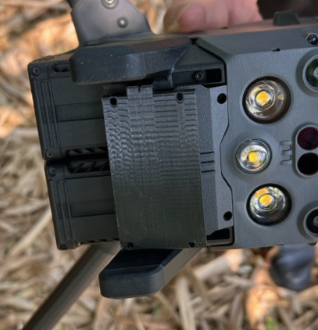
\includegraphics[width=\linewidth]{fig/3D+Drone.png}
        \small (a) โครงยึดอุปกรณ์ก่อนติดตั้งโมดูล UWB
    \end{minipage}
    \hfill
    \begin{minipage}{0.45\textwidth}
        \centering
        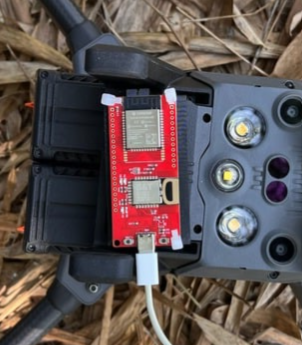
\includegraphics[width=\linewidth]{fig/3D+UWB.png}
        \small (b) การติดตั้งโมดูล UWB บนโดรน
    \end{minipage}

    \caption{ขั้นตอนการติดตั้งโมดูล UWB บนโดรน}
    \label{fig:uwb-installation}
\end{figure}

\section{โครงสร้างซอฟต์แวร์ของระบบ}
\begin{enumerate}
    \item \textbf{UWB Program:} เป็นโปรแกรมที่พัฒนาบน ESP32 สำหรับควบคุมการทำงานของโมดูล UWB ในการวัดระยะทางระหว่าง Tag และ Anchor รวมถึงการส่งข้อมูลระยะทางไปยังระบบบันทึกข้อมูล
    \item \textbf{Data Logging (CSV):} ใช้สำหรับบันทึกข้อมูลที่ได้จากการวัด เช่น ระยะทางจาก UWB และข้อมูลจากโดรน โดยทำการจัดรูปแบบข้อมูลตามลำดับเวลา และบันทึกในรูปแบบไฟล์ CSV เพื่อใช้ในการวิเคราะห์
    \item \textbf{WebODM:} ใช้สำหรับประมวลผลภาพถ่ายทางอากาศจากโดรน เพื่อสร้างแบบจำลองสามมิติ (3D Model) และข้อมูล Point Cloud สำหรับใช้ในการคำนวณความสูงของต้นไม้
\end{enumerate}

\section{ขั้นตอนการดำเนินงาน (Workflow)}

การดำเนินงานของระบบในการทดลองภาคสนามสามารถอธิบายได้ตามลำดับขั้นตอนดังนี้

\begin{enumerate}
    \item ใช้โดรนบินเก็บภาพถ่ายทางอากาศของพื้นที่เพื่อใช้ในการสร้างแบบจำลองสามมิติ
    \item ทำการติดตั้ง Anchor บนพื้นดินใต้ต้นไม้เป้าหมาย และเตรียมระบบรับข้อมูล
    \item นำโดรนลงจอดและติดตั้งโมดูล UWB Tag บนโครงยึดใต้โดรน
    \item บินโดรนขึ้นไปลอยตัวเหนือยอดไม้ เพื่อวัดระยะจากโดรนถึงยอดไม้ด้วยเซ็นเซอร์ VPS
    \item รักษาระดับความสูงเดิม และเคลื่อนที่ในแนวราบเพื่อจัดตำแหน่งให้เหมาะสมสำหรับการวัดระยะด้วย UWB
    \item ทำการวัดระยะระหว่าง Tag และ Anchor ด้วยเทคนิค ToF
    \item บันทึกข้อมูลระยะทางทั้งหมดลงในระบบ
    \item ประมวลผลภาพถ่ายด้วย WebODM เพื่อสร้าง 3D Point Cloud
    \item คำนวณความสูงของต้นไม้จากทั้งสองวิธี
    \item เปรียบเทียบผลลัพธ์เพื่อประเมินความแม่นยำของระบบ
\end{enumerate}

\section{วิธีการคำนวณความสูงของต้นไม้}

\subsection{การคำนวณจาก UWB และ VPS}

ความสูงของต้นไม้สามารถประมาณได้จากผลต่างของระยะทางที่วัดได้จากระบบ UWB และเซ็นเซอร์ VPS ดังสมการ

\begin{equation}
H_{tree} = D_{UWB} - D_{VPS}
\end{equation}

โดยที่

\begin{itemize}
    \item $H_{tree}$ คือ ความสูงของต้นไม้
    \item $D_{UWB}$ คือ ระยะห่างระหว่าง Tag และ Anchor
    \item $D_{VPS}$ คือ ระยะจากโดรนถึงยอดไม้
\end{itemize}

\subsection{การคำนวณความสูงจากแบบจำลองสามมิติ}
ความสูงของต้นไม้จากแบบจำลองสามมิติถูกวัดโดยใช้เครื่องมือวัดระยะภายในซอฟต์แวร์ WebODM ซึ่งอาศัยข้อมูลจาก 3D Point Cloud ที่สร้างขึ้นจากภาพถ่ายทางอากาศ โดยทำการเลือกจุดที่แทนตำแหน่งยอดไม้ และจุดที่แทนระดับพื้นดิน จากนั้นคำนวณระยะห่างในแนวดิ่งระหว่างสองจุดดังกล่าวเพื่อประมาณค่าความสูงของต้นไม้
